\section{Auswertung}
\label{sec:Auswertung}
Die Schallgeschwindigkeiten in Wasser und Acryl sind durch
\begin{align*}
  c_{\symup{Acryl}} &= 2730\,\unit{\meter\per\second}\\
  c_{\symup{Luft}}  &= 1480\,\unit{\meter\per\second}
\end{align*}
gegeben \cite{schallgeschwindigkeit}.

\subsection{Maße des Acrylbocks}
Die Messung ergibt für die Länge $l$ und Höhe $h$ des Acrylblocks.
\begin{align*}
  \symup{l} &= 15,028\,\unit{\centi\meter}\\
  \symup{h} &= 8,025\,\unit{\centi\meter}.
\end{align*}
Die Messwerte für die Lage und Größe der Löcher sind in \autoref{tab:Abstand_Durchmesser} zu finden.
\begin{table}
  \centering
  \begin{tabular}{c c c}
    \toprule
    Störstelle & $\symup{s}/\unit{\centi\meter}$ & $\symup{d}/\unit{\centi\meter}$\\
    \midrule
    $\symup{c}_{\symup{1}}$ & $6,180$ & $0,145$ \\
    $\symup{c}_{\symup{2}}$ & $6,060$ & $0,145$ \\
    $\symup{a}_{\symup{1}}$ & $1,505$ & $0,565$ \\
    $\symup{a}_{\symup{2}}$ & $2,385$ & $0,490$ \\
    $\symup{a}_{\symup{3}}$ & $3,220$ & $0,400$ \\
    $\symup{a}_{\symup{4}}$ & $3,980$ & $0,385$ \\
    $\symup{a}_{\symup{5}}$ & $4,880$ & $0,300$ \\
    $\symup{a}_{\symup{6}}$ & $5,595$ & $0,260$ \\
    $\symup{a}_{\symup{7}}$ & $6,390$ & $0,290$ \\
    $\symup{a}_{\symup{8}}$ & $7,210$ & $0,270$ \\
    $\symup{b}            $ & $1,945$ & $0,975$ \\
    \bottomrule
  \end{tabular}
  \caption{Abstand und Durchmesser der Löcher von der unteren Kante aus gemessen.}
  \label{tab:Abstand_Durchmesser}
\end{table}
Die Messwerte können zum Abgleich mit den Ergebnissen der Ultraschallmessung verwendet werden.

\subsection{}

\begin{figure}
  \centering
  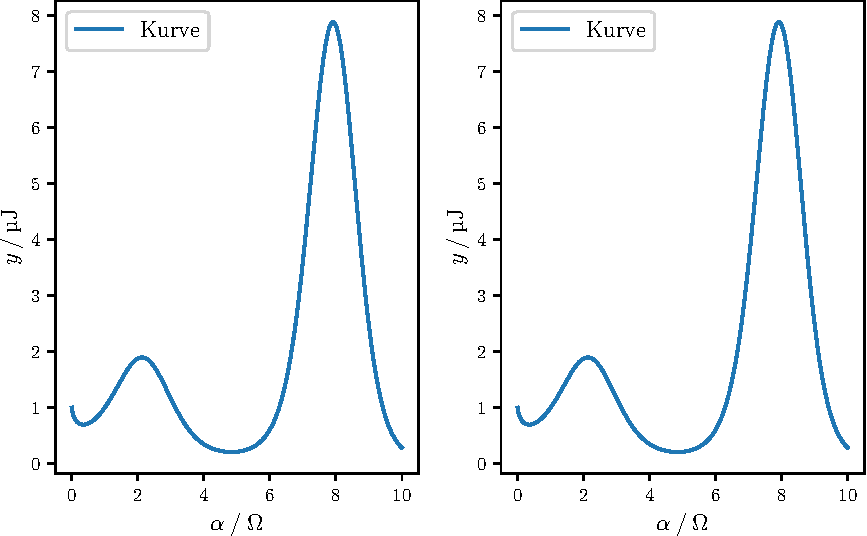
\includegraphics{plot.pdf}
  \caption{Plot.}
  \label{fig:plot}
\end{figure}

